\begin{frame}{}
    \begin{center}
        \LARGE Simulación
    \end{center}
\end{frame}

\begin{frame}{Simulación}

\begin{itemize}
    \item Para estudiar el modelo Dark-SUSY de forma experimental y caracterizar las propiedad de la se\~nal  
    se requiere generar muestras de simulación por el método de Monte Carlo 
    \item La simulación requiere generar varias muestras considerando los parámetros m\'as importantes del fotón oscuro (masa y tiempo de vida) 
    \item Para generar las muestras simuladas se hace uso de paquetes propios del área de altas energías, los cuales actúan de forma sequencial y se encargan de diferentes aspectos del proceso de análisis. 
\end{itemize}
    
\end{frame}


\begin{frame}{Paquetes de Simulación}
\begin{itemize}
    \item \textbf{Madgraph}: Se encarga de procesar la informaci\'on fundamental del modelo como la masa de las particulas madre, diagramas de Feynman, amplitudes de decaimiento, etc. 
    \item \textbf{Pythia}: Se encarga del proceso de hadronización, es decir la interacción entre protones, recombinación de quarks y formación de nuevas partículas 
    \item \textbf{Delphes}: Se encarga de simular la respuesta del detector al paso de las partículas simuladas, en este paso se consideran eficiencia de detecciones y se extraen variables como la energia, momento y trayectoria reconstruida de las partículas en cuestión
\end{itemize}

\end{frame}

\begin{frame}{Estrategia de Simulación}

\begin{itemize}
    \item Para generar las muestras se requiere crear un entorno automatizado (python) el cual pueda ser flexible a las diferentes variaciones del modelo
    \item Los archivos resultantes (formato .root) contienen la informaci\'on (teorica+experimental) para realizar el an\'alisis de datos.  
\end{itemize}

\begin{figure}[h]
\centering
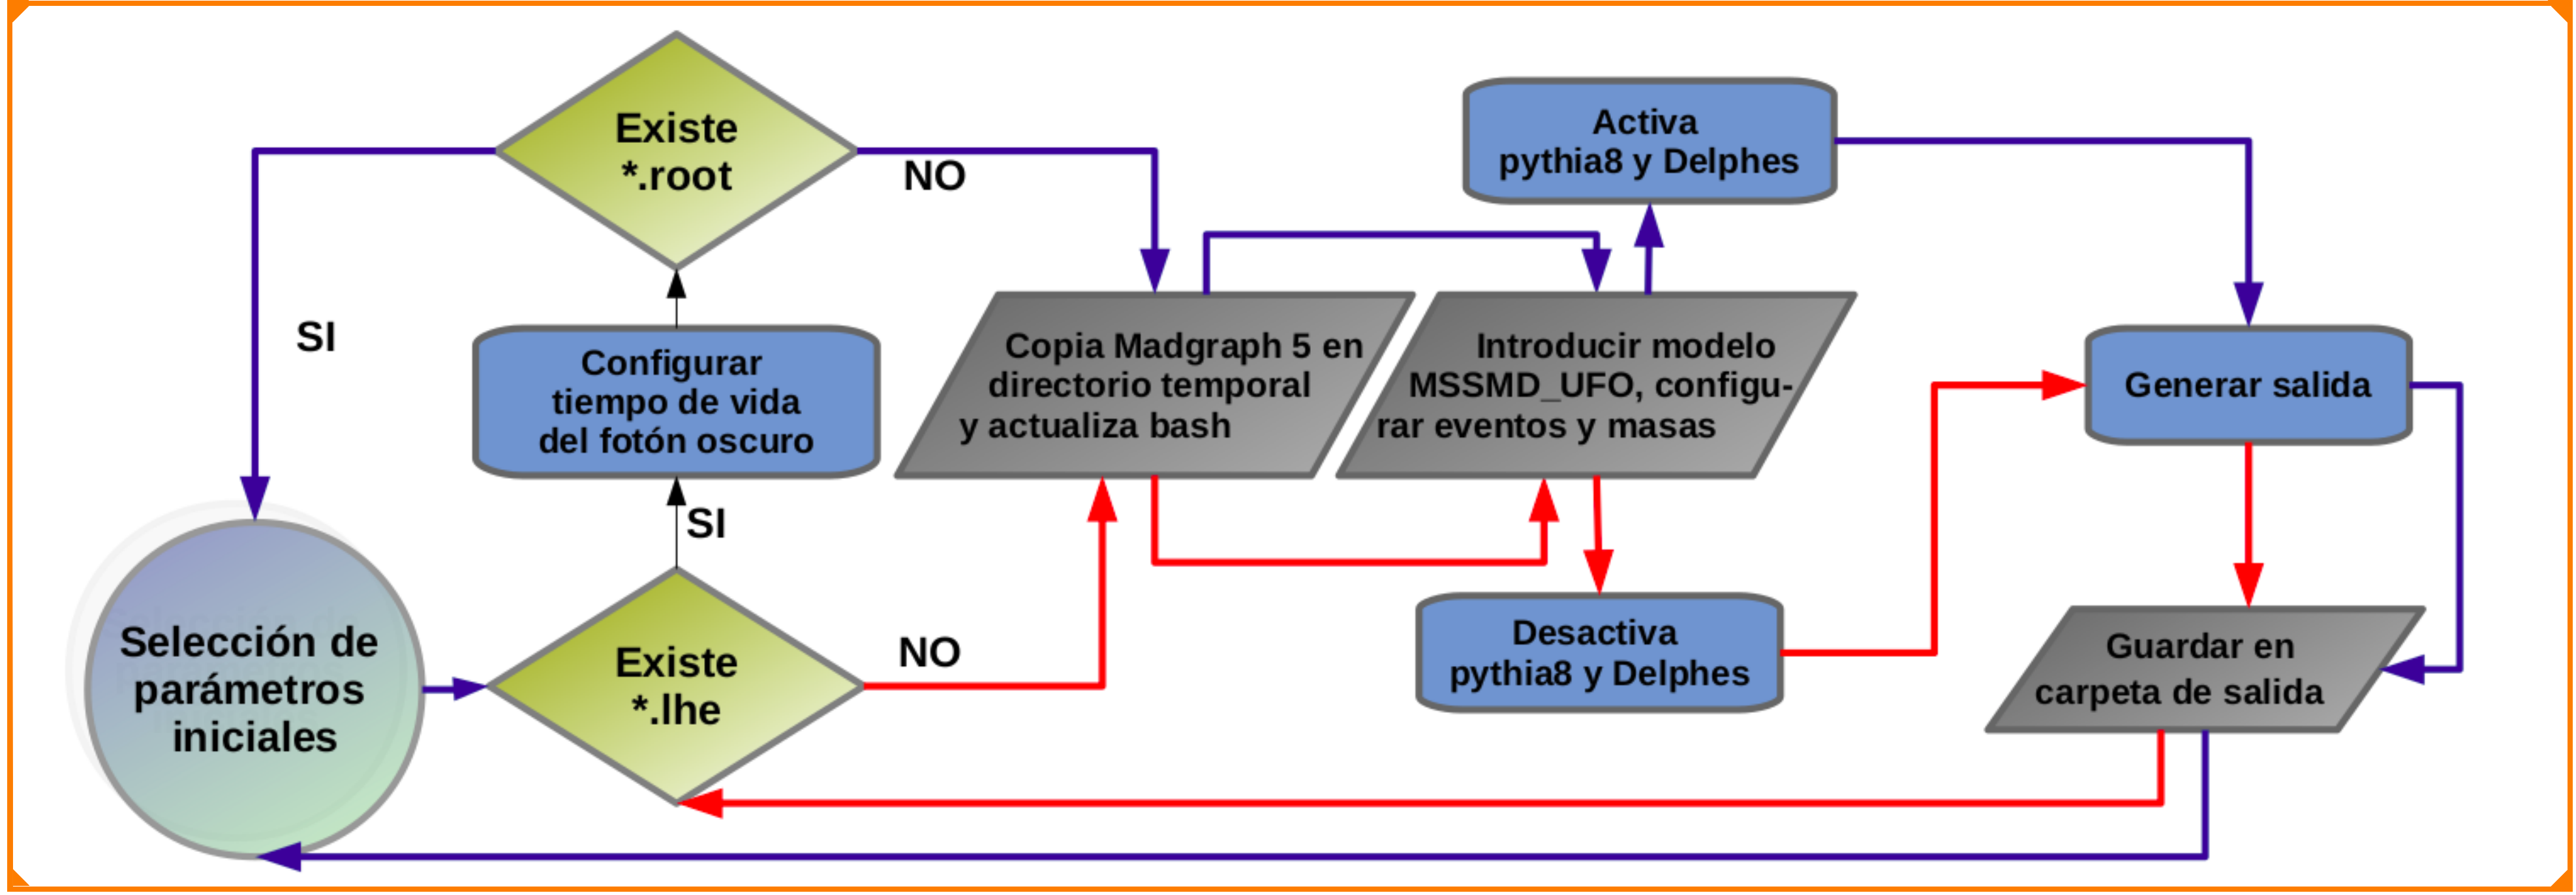
\includegraphics[width=0.8\textwidth]{Imag/proyecto_darksusy2.png}
\caption{Diagrama de Flujo del generador.}
\end{figure}

%Incluir diagrama donde se describa como se inicia la simulacion Madgraph->Pythia->Delphes
    
\end{frame}


\begin{frame}{Muestras simuladas}
    \begin{itemize}
        \item Para generar cada muestra se requiere especificar los siguientes parámetros: masa del neutralino ($m_{n_{1}}$), masa del dark neutralino ($m_{n_{D}}$), masa del fotón oscuro ($m_{\gamma_{D}}$) y tiempo de vida del foton oscuro ($c\tau_{\gamma_{D}}$) que son los parámetros del modelo Dark-SUSY. 
        %\item El numero de muestras simuladas se representa en la siguiente tabla
        \item El número de muestras simuladas es el resultado de todas las combinaciones posibles de los vectores correspondientes a los parámetros de generación, haciendo un total de $\backsim 15 000$ muestras:
    \end{itemize}

\begin{table}
\begin{footnotesize}
\begin{tabular}{|cl|}
\hline
$V_{m_{n_{1}}}$ & = $[10, ~20, ~30, ~40, ~50, ~60, ~70, ~80, ~90, ~100]$\\
$V_{m_{n_{D}}}$ & = $[0.25, ~1, ~2, ~3, ~4, ~5, ~10]$\\
$V_{m_{\gamma_{D}}}$ & = $[0.25, ~1, ~2, ~3, ~4, ~5, ~6, ~7, ~8, ~9, ~10]$\\
$V_{c\tau_{\gamma_{D}}}$ & = $[0, ~1, ~2, ~3, ~4, ~5, ~10, ~20, ~30, ~40, ~50, ~100]$\\
Eventos simulados &  = 10000\\
\hline
\hline
\end{tabular}
\end{footnotesize}
\end{table}

    
%\begin{table}
%\begin{footnotesize}
%\begin{tabular}{|ccccc|}
%\hline
%$m_{n_{1}}$ & $m_{n_{D}}$ & $m_{\gamma_{D}}$ & $c\tau_{\gamma_{D}}$ & Eventos simulados \\
%\hline
%\hline
%\end{tabular}
%\end{footnotesize}
%\end{table}

    

\end{frame}






\begin{comment}

\begin{frame}{Muestras simuladas}
Notación:\\
$\mathbb{E}_i^{(j,~k)} ~= ~1$  hace referencia a los eventos, donde $i = \{1, \ldots, i_{max}\}$ corresponde al elemento del evento en el árbol de archivo $*.root$ requerido, y donde: $\{j, ~k\} = \{\{0\mu, ~1\mu, ~2\mu, ~3\mu, ~4\mu\, \ldots\},\{\mathtt{CMS},~\mathtt{HL}\}\}$ hace referencia a los eventos según su contenido muónico y al detector que generó los datos. Entonces:
\begin{equation*}
\mathbb{E}^{(j,~\mathtt{CMS})} = \sum_i \mathbb{E}_i^{(j, ~\mathtt{CMS})} , ~~~~ \mathbb{E}_i^{(\mathtt{CMS})} = \sum_j \mathbb{E}_i^{(j,~\mathtt{CMS})} ~~~~ y ~~~~ \mathbb{E}^{\mathtt{(CMS)}}= \sum_{ij} \mathbb{E}_i^{(j,~\mathtt{CMS})}
\end{equation*}
\begin{equation*}
\mathbb{E}^{(j,~\mathtt{HL})} = \sum_i \mathbb{E}_i^{(j, ~\mathtt{HL})} , ~~~~ \mathbb{E}_i^{(\mathtt{HL})} = \sum_j \mathbb{E}_i^{(j,~\mathtt{HL})} ~~~~ y ~~~~ \mathbb{E}^{\mathtt{(HL)}}= \sum_{ij} \mathbb{E}_i^{(j,~\mathtt{HL})}
\end{equation*}
donde:
\begin{equation*}
\mathbb{E}^{(j,~k)}\equiv \mathbb{E}^{(j,~k)}\mathtt{(MNeuL,~MNeuD,~MPhoD,~TcPhoD)}
\end{equation*}

\end{frame}



\begin{frame}{Muestras simuladas}
Notación:\\
\begin{equation*}
f^{(j,~k)} = \dfrac{\mathbb{E}^{(j,~k)}}{\mathbb{E}^{(k)}}
\end{equation*}
Para el caso que nos ocupa $\mathbb{E}^{(k)} ~= ~\mathtt{Event} ~= ~10 000$ son los eventos simulados para cada configuración requerida. Ejemplos:
\begin{table}
\begin{footnotesize}
\begin{tabular}{|cccccc|}
\hline
$\texttt{MNeuL(GeV)}$ & $\texttt{MNeuD(GeV)}$ & $\texttt{MPhoD(GeV)}$ & $\texttt{TcPhoD(mm)}$ & $f^{(4\mu,~\texttt{CMS})}$ & $f^{(4\mu,~\texttt{HL})}$ \\
\hline
10 & 0.25 & 0.25 & 0.5 & 0.0920 & 0.1678\\
& & & 2 & 0.0779 & 0.1355 \\
& & & 4 & 0.0597 & 0.1024 \\
& & & 10 & 0.0227 & 0.0433 \\
& & & 50 & 0.0016 & 0.0039 \\
\hline
10 & 0.25 & 0.25 & 2 & 0.0497 & 0.1135 \\
& & 4 & & 0.0494 & 0.1157 \\
& & 6 & & 0.0599 & 0.1456 \\
& & 8 & & 0.0957 & 0.1960 \\
\hline
\end{tabular}
\end{footnotesize}
\end{table}

%\begin{table}[]
%    \centering
%    \begin{tabular}{c|c|c|}  \hline
%    Masa [GeV]     & Tiempo de vida [mm]  &  Numero de eventos \\ \hline 
%         &  & \\ \hline 
%         & & \\ \hline 
%    \end{tabular}
%    \caption{Muestras simuladas del modelo Dark-SUSY}
%    \label{tab:my_label}
%\end{table}
    
\end{frame}
\end{comment}


\begin{frame}{Simulaci\'on del Detector en Delphes}

\begin{itemize}
    \item Delphes es un paquete de simulaci\'on rapida, es decir alguna de las eficiencias de deteccion estan parametrizadas, lo anterior para reducir el tiempo de simulaci\'on 
    \item Dichar parametrizaciones se obtienen de la simulaci\'on mas detallada (Geant4) la cual contempla todos los procesos fundamentales del paso de las particulas por el detector
    \item En nuestro modelo los fotones oscuros decaen a muones, por lo que la reconstrucci\'on de los mismos es parte fundamental del an\'alisis
\end{itemize}
\end{frame}

\begin{frame}{Identificación de muones en CMS}
    
\begin{itemize}
  
    \item Los muones son particulas elementales que interaccionan débilmente con la materia, su trayectoria se reconstruye con informaci\'on obtenida de detectores dedicados a esta tarea
    \item A partir de la trayectoria reconstruida y la desviaci\'on provocada por el campo magn\'etico solenoide se puede obtener el valor del momento.
    \tiem Debido a que el fotón oscuro puede viajar una distancia considerable antes de decaer la eficiencia de reconstrucción de muones esta íntimamente ligado al tiempo de vida (c$\tau$) 
    \item En general se espera que a mayor tiempo de vida del fotón oscuro la eficiencia de identificación es menor (debido a que los muones logran atravesar solo una parte de los dispositivos de detección)
\end{itemize}
\end{frame}

\begin{frame}{Identificación de muones en CMS}

\begin{itemize}
    \item La linea azul representa el paso de los muones por el detector CMS
\end{itemize}

\begin{figure}
    \centering
    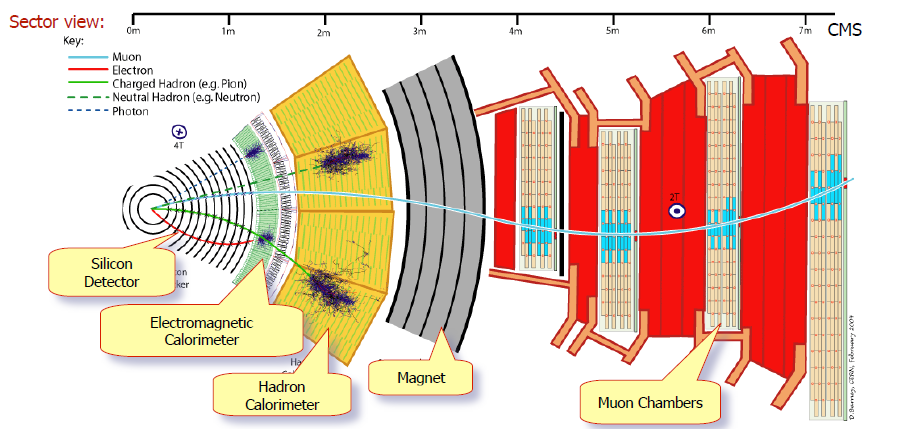
\includegraphics[scale=0.35]{Imag/reconstruccion_muones.png}
    \caption{Identificación de partículas en CMS, vista transversal del detector}
    \label{fig:my_label}
\end{figure}
    
\end{frame}

\begin{frame}{Definición de variables relevantes}

El detector CMS tiene una simetría cilindrica en donde el eje de colisi\'on es el "z" y el plano transversal esta formado por los ejes "x" e "y". Dos de las variables para caracterizar las propiedades de las partículas son las siguientes. 

    \begin{figure}[ht]
        \begin{minipage}[b]{0.45\linewidth}
            \centering
            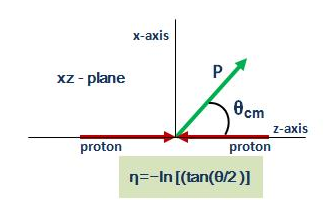
\includegraphics[width=\textwidth]{pseudorapidity.PNG}
            \caption{Definición de pseudorapidez}
            \label{fig:a}
        \end{minipage}
        \hspace{0.5cm}
        \begin{minipage}[b]{0.45\linewidth}
            \centering
            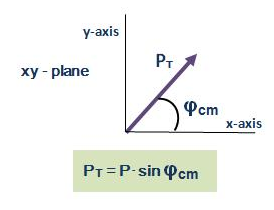
\includegraphics[width=\textwidth]{pt.PNG}
            \caption{Definición de momento transversal}
            \label{fig:b}
        \end{minipage}
    \end{figure}
    
\end{frame}

\begin{frame}{Parametrización de eficiencia y resolución}

Estas parametrizaci\'on est\'an contenidas en la simulaci\'on Delphes

%\color{red} Francisco aqui poner las graficas de eficiency y resolucion que habiamos obtenido examinando los datacards de Delphes, hacerlo para el detector actual (no HL-LHC)

    \begin{figure}[ht]
        \begin{minipage}[b]{0.45\linewidth}
            \centering
            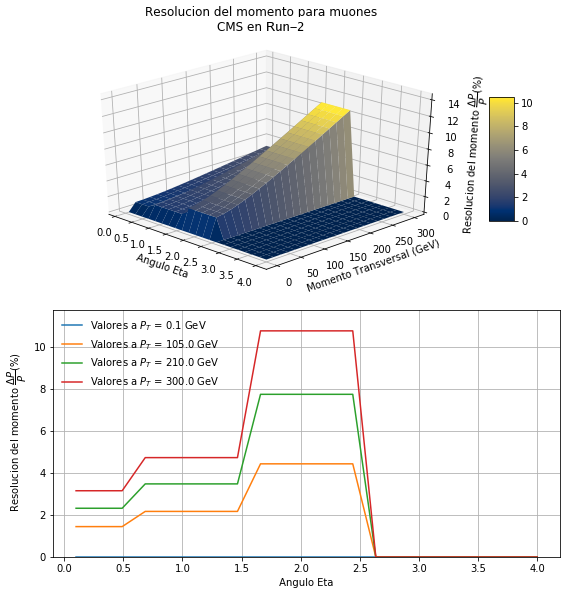
\includegraphics[width=\textwidth]{Imag/Momentum_resolution_of_Muon_CMS.png}
            \caption{Resolución del momento para muones.}
            \label{fig:a}
        \end{minipage}
        \hspace{0.5cm}
        \begin{minipage}[b]{0.45\linewidth}
            \centering
            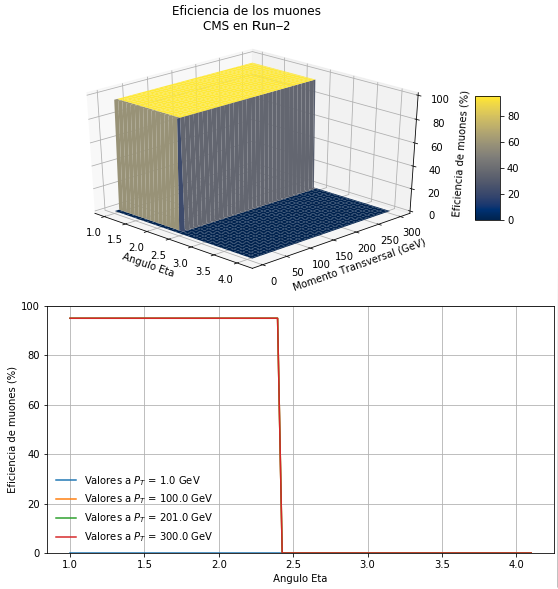
\includegraphics[width=\textwidth]{Imag/Eficiencia_of_Muon_CMS.png}
            \caption{Eficiencia en la reconstrucción de los muones.}
            \label{fig:b}
        \end{minipage}
    \end{figure}
    
\end{frame}